
In the demonstration we show a play of some variant of the game Hanabi. 
In this game, each agent has cards with a color and a
number, but cannot see his own hand.
In each turn, the user can play the role of one of the agent: he/she can either give the information to some other agent about a number or a color, or play a card. The goal is to play the cards in increasing order for each color.
During the process, the system keeps track on the knowledge of the agents.
More precisely, the system shows the real world (the real distribution of the cards). When the user clicks on an agent, it displays a \emph{sampling} of some possible worlds for that agent (some possible distributions of cards he/she still consider as possible at some stage of the game). The agents also reason about knowledge of other agents, see in Figure~\ref{figure:guihanabi} (two levels of knowledge are shown).
%
%
%% expliquer la démo. Je me suis peut etre trompé sur le nombre de cartes ici et si on gère les jetons pour les infos il faut le mettre dans le paragraphe.
%


\begin{figure}
	\begin{center}
		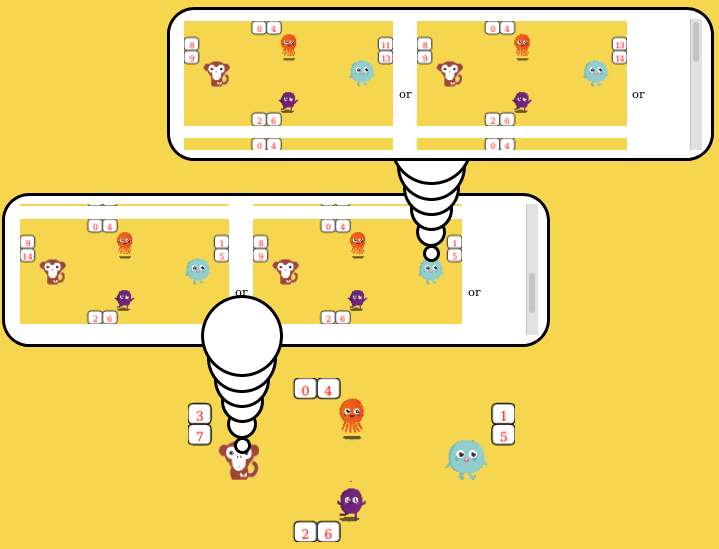
\includegraphics[width=4cm]{images/HW_screenshot_hanabi.png}
	\end{center}
\vspace{-3mm}
	\caption{Screenshot of Hanabi in \emph{Hintikka's World}.\label{figure:guihanabi}}
\end{figure}
%%\newpage

Note that in this demonstration, in order to explain models of DEL, the tool still presents examples that rely on explicit models, such as Sally and Anne, muddy children, consecutive numbers, etc.